\documentclass{beamer}
\usepackage{beamerthemesplit}
\usepackage{wrapfig}
\usetheme{SPbGU}
\usepackage{pdfpages}
\usepackage{amsmath}
\usepackage{cmap} 
\usepackage[T2A]{fontenc} 
\usepackage[utf8]{inputenc}
\usepackage[english,russian]{babel}
\usepackage{indentfirst}
\usepackage{amsmath}
\usepackage{tikz}
\usepackage{multirow}
\usepackage[noend]{algpseudocode}
\usepackage{algorithm}
\usepackage{algorithmicx}
\usepackage{epstopdf}
\usetikzlibrary{shapes,arrows}
\usepackage{fancyvrb}
\newtheorem{rutheorem}{Theorem}
\newtheorem{ruproof}{Доказательство}
\newtheorem{rudefinition}{Определение}
\newtheorem{rulemma}{Лемма}
\beamertemplatenavigationsymbolsempty

\title[]{Relaxed Parsing of Regular Approximations of String-Embedded Languages}
%\subtitle[]{В рамках проекта лаборатории JetBrains}
\institute[SPbSU]{
Saint Petersburg State University \\
JetBrains Programming Languages and Tools Lab }

\author[Ekaterina Verbitskaia]{Ekaterina Verbitskaia
% \\
%  \and  
%    {\bfseries Научный руководитель:} ст.пр. С.В. Григорьев \\ 
%  \and
%    {\bfseries Рецензент:} программист "ИнтеллиДжей Лабс" А.А. Бреслав 
}

\date{26/08/2015}

\definecolor{orange}{RGB}{179,36,31}

\begin{document}
{

\begin{frame}
  \begin{center}
  {
\includegraphics[width=1cm]{SPbGU_Logo.png}}
  \end{center}
  \titlepage
\end{frame}
}

\begin{frame}[fragile]
  \transwipe[direction=90]
  \frametitle{String embedding}
  \begin{itemize}
    \item Dynamic SQL
      \begin{Verbatim}[commandchars=\\\{\}]
\textcolor{blue}{IF} @X = @Y
    \textcolor{blue}{SET} @TBL = \textcolor{orange}{' #table1 '}
\textcolor{blue}{ELSE}
    \textcolor{blue}{SET} @TBL = \textcolor{orange}{' table2 '}
\textcolor{blue}{SET} @S = \textcolor{orange}{'SELECT x FROM'} + @TBL + \textcolor{orange}{'WHERE ISNULL(n,0) > 1'}
EXECUTE (@S)
       \end{Verbatim}
    \item Embedded SQL
      \begin{Verbatim}[commandchars=\\\{\}]
\textcolor{blue}{SqlCommand} myCommand = new \textcolor{blue}{SqlCommand}(
    \textcolor{orange}{"SELECT * FROM table WHERE Column = @Param2"},
    myConnection);
myCommand.Parameters.Add(myParam2);
      \end{Verbatim}
    \end{itemize}
\end{frame}

\begin{frame}
  \transwipe[direction=90]
  \frametitle{Problems}  
  \begin{itemize}
    \item String-embedded code are expressions in some programming language
    \begin{itemize}
      \item It may be necessary to support them in IDE: code highlighting, 
autocomplete, refactorings
      \item It may be necessary to transform them: migration of legacy software 
on new platforms
      \item It may be necessary to detect vulnerabilities in such code
      \item Any other problems of programming languages can occur
    \end{itemize}
  \end{itemize}
\end{frame}

\begin{frame}
  \transwipe[direction=90]
  \frametitle{Static analysis of string-embedded code}  
  \begin{itemize}
    \item Performed without programm execution
    \item Checks that the set of properties holds for each possible expression value
  \end{itemize}
  
  \begin{itemize}
    \item Undecidable for string-embedded code in the general case
    \item The set of possible expression values is over approximated and then 
the approximation is analysed.
  \end{itemize}
\end{frame}

\begin{frame}
  \transwipe[direction=90]
  \frametitle{Static analysis of string-embedded code: the scheme}
  \begin{itemize}
    \item Identification of hotspots: points of interest, where the analysis is 
desirable
    \item Approximation construction
    \item Lexical analysis
    \item \textbf{Syntactic analysis}
    \item Semantic analysis
  \end{itemize}
\end{frame}



\begin{frame}[fragile]
\transwipe[direction=90]
\frametitle{Static analysis of string-embedded code: the scheme}

\begin{tabular}{p{4.5cm} p{8cm}}
Code: hotspot is marked
&
\begin{minipage}[t]{5cm}

\begin{Verbatim}[commandchars=\\\{\}]
\textcolor{blue}{string} res = \textcolor{orange}{""};
\textcolor{blue}{for}(i = 0; i < l; i++)
    res = \textcolor{orange}{"()"} + res;
\fbox{\textcolor{blue}{use}(res);}

\end{Verbatim}
\end{minipage}

\\ 
Possible values
&
\begin{minipage}[t]{2.5cm}
\begin{Verbatim}[commandchars=\\\{\}]
\{\textcolor{orange}{""}, \textcolor{orange}{"()"},  \textcolor{orange}{"()()"}, ..., \textcolor{orange}{"()"}^l\}
\end{Verbatim}
\end{minipage}

\\
Regular approximation
&
\begin{minipage}[t]{4cm}
  \begin{Verbatim}[commandchars=\\\{\}]
(\textcolor{orange}{"()"})*
  \end{Verbatim} 
\end{minipage}

\\
Approximation
&
\begin{minipage}[t]{3cm}
\raisebox{-\height}{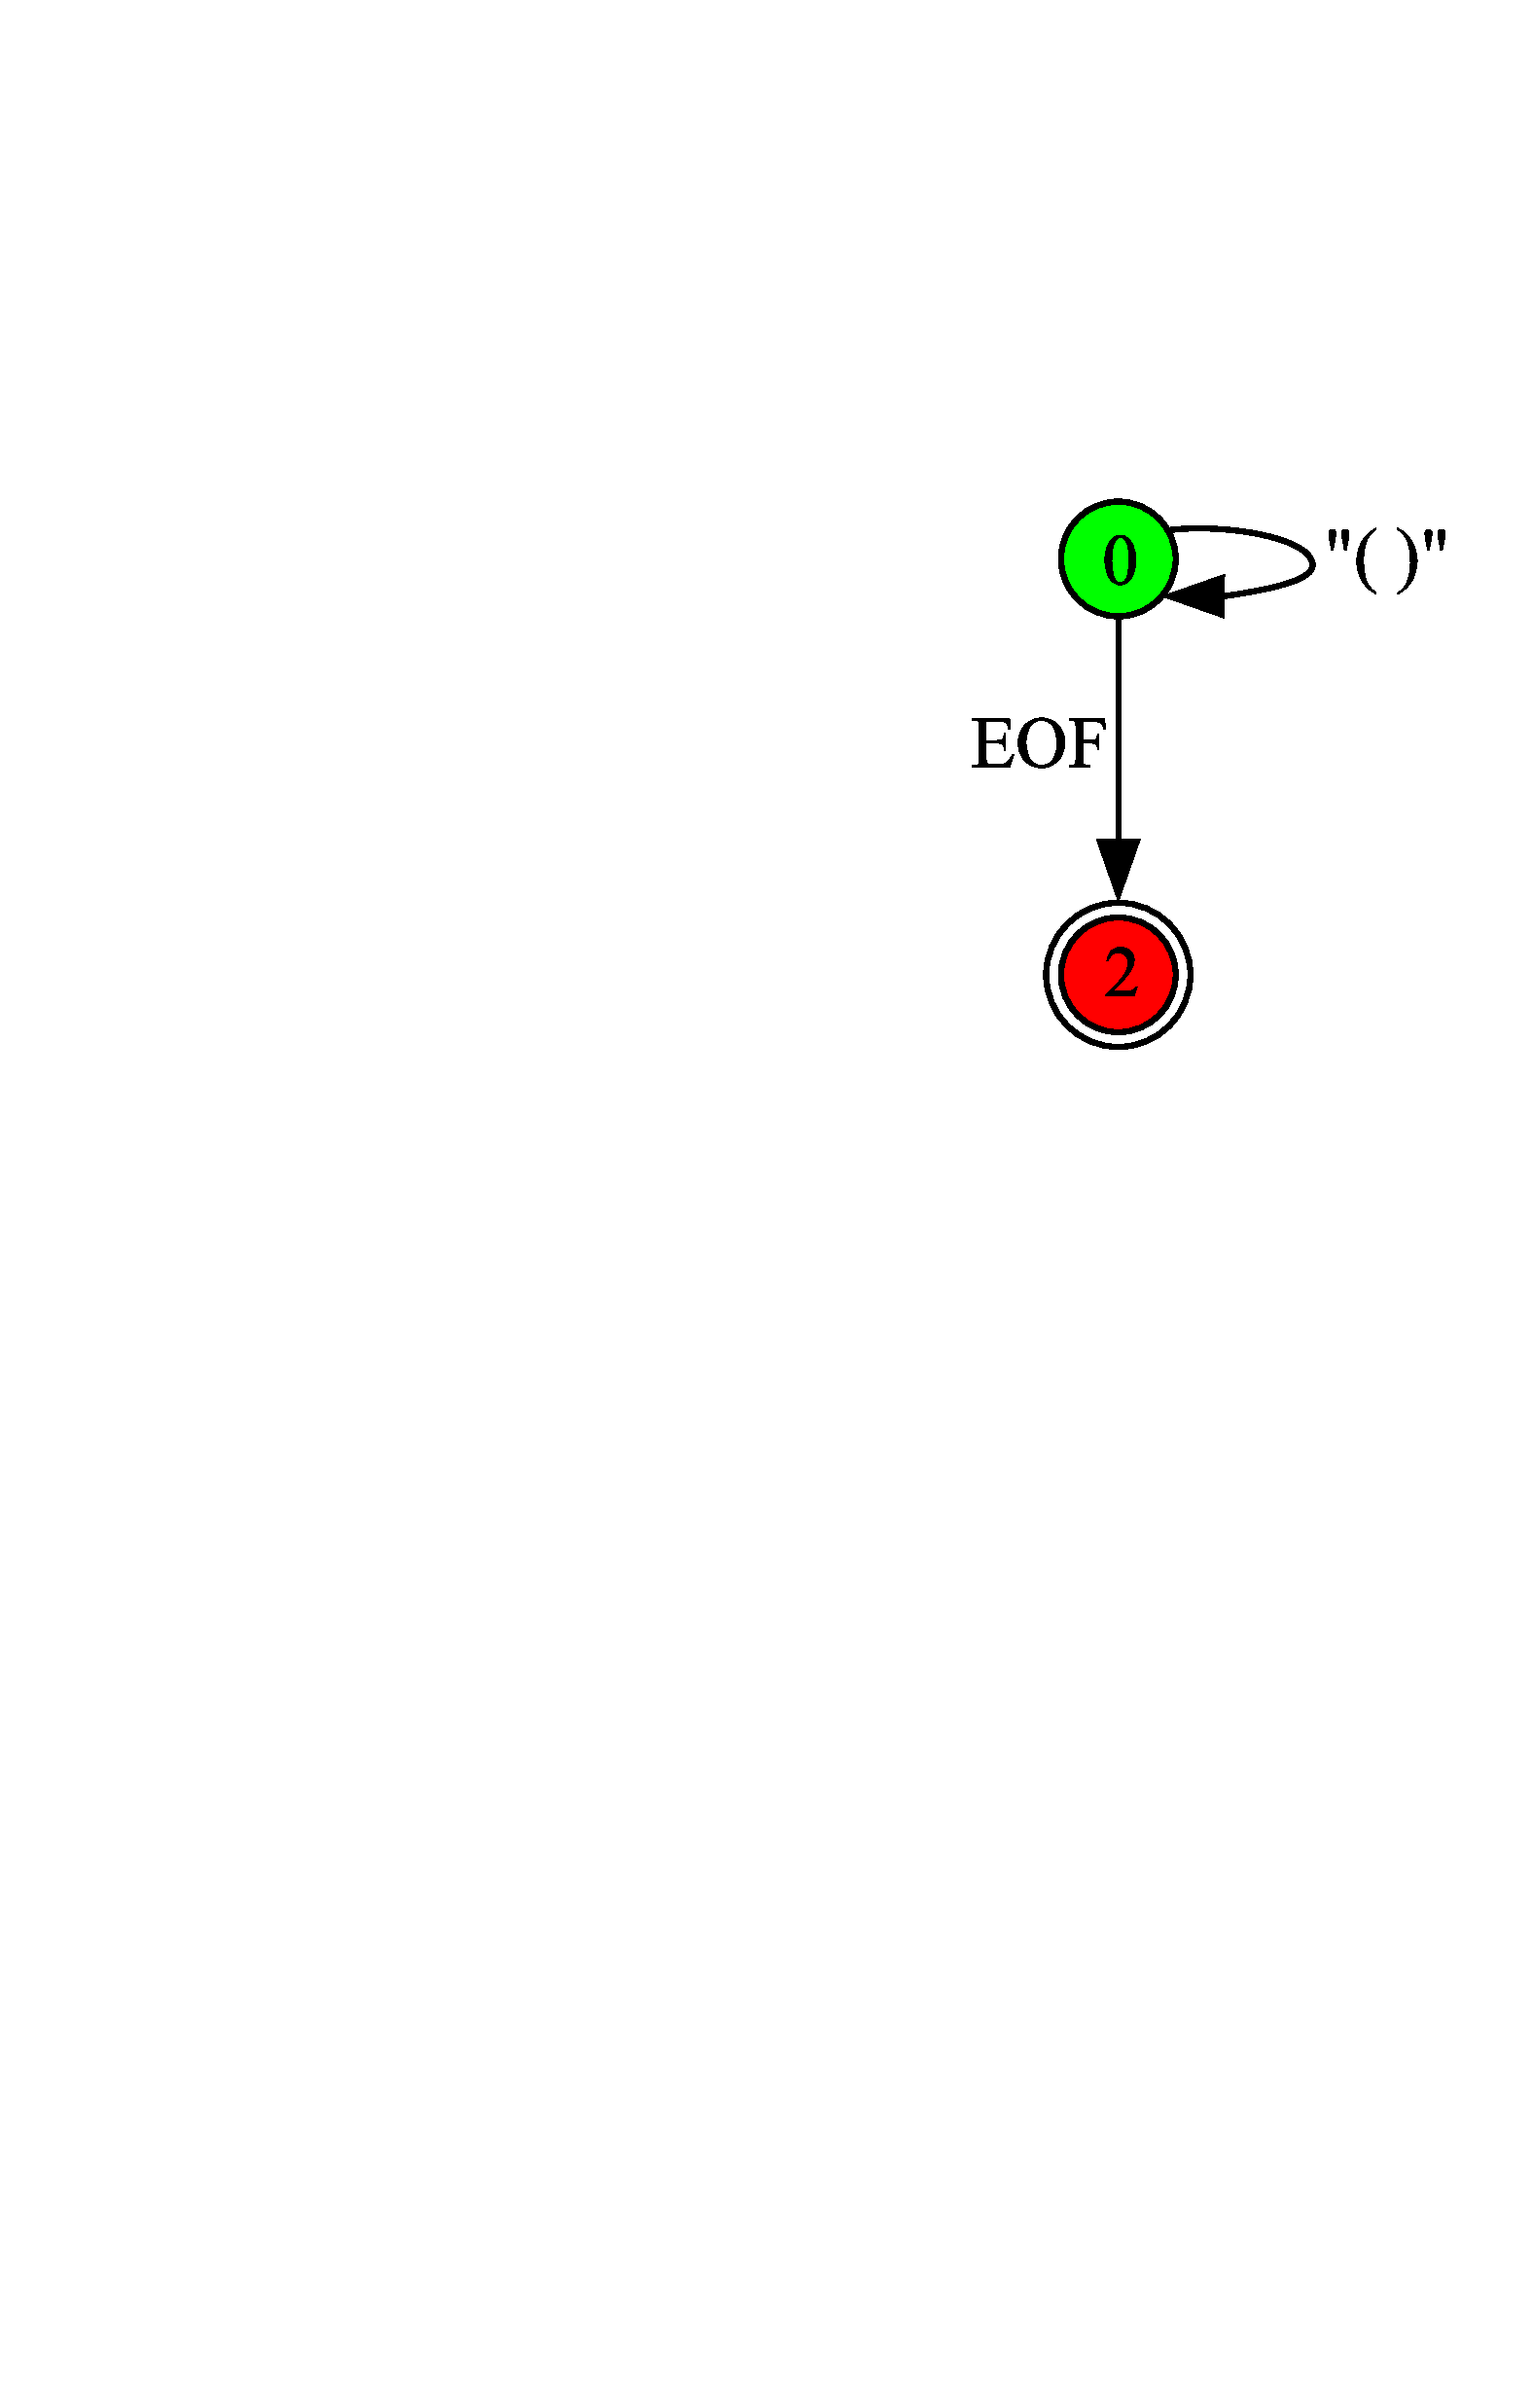
\includegraphics[width=2cm]{pictures/lex1}}
\end{minipage}


\end{tabular}


\end{frame}


\begin{frame}[fragile]
\transwipe[direction=90]
\frametitle{Static analysis of string-embedded code: the scheme}

\begin{tabular}{p{4.5cm} p{8cm}}
\begin{minipage}[t]{4cm}
Approximation\\
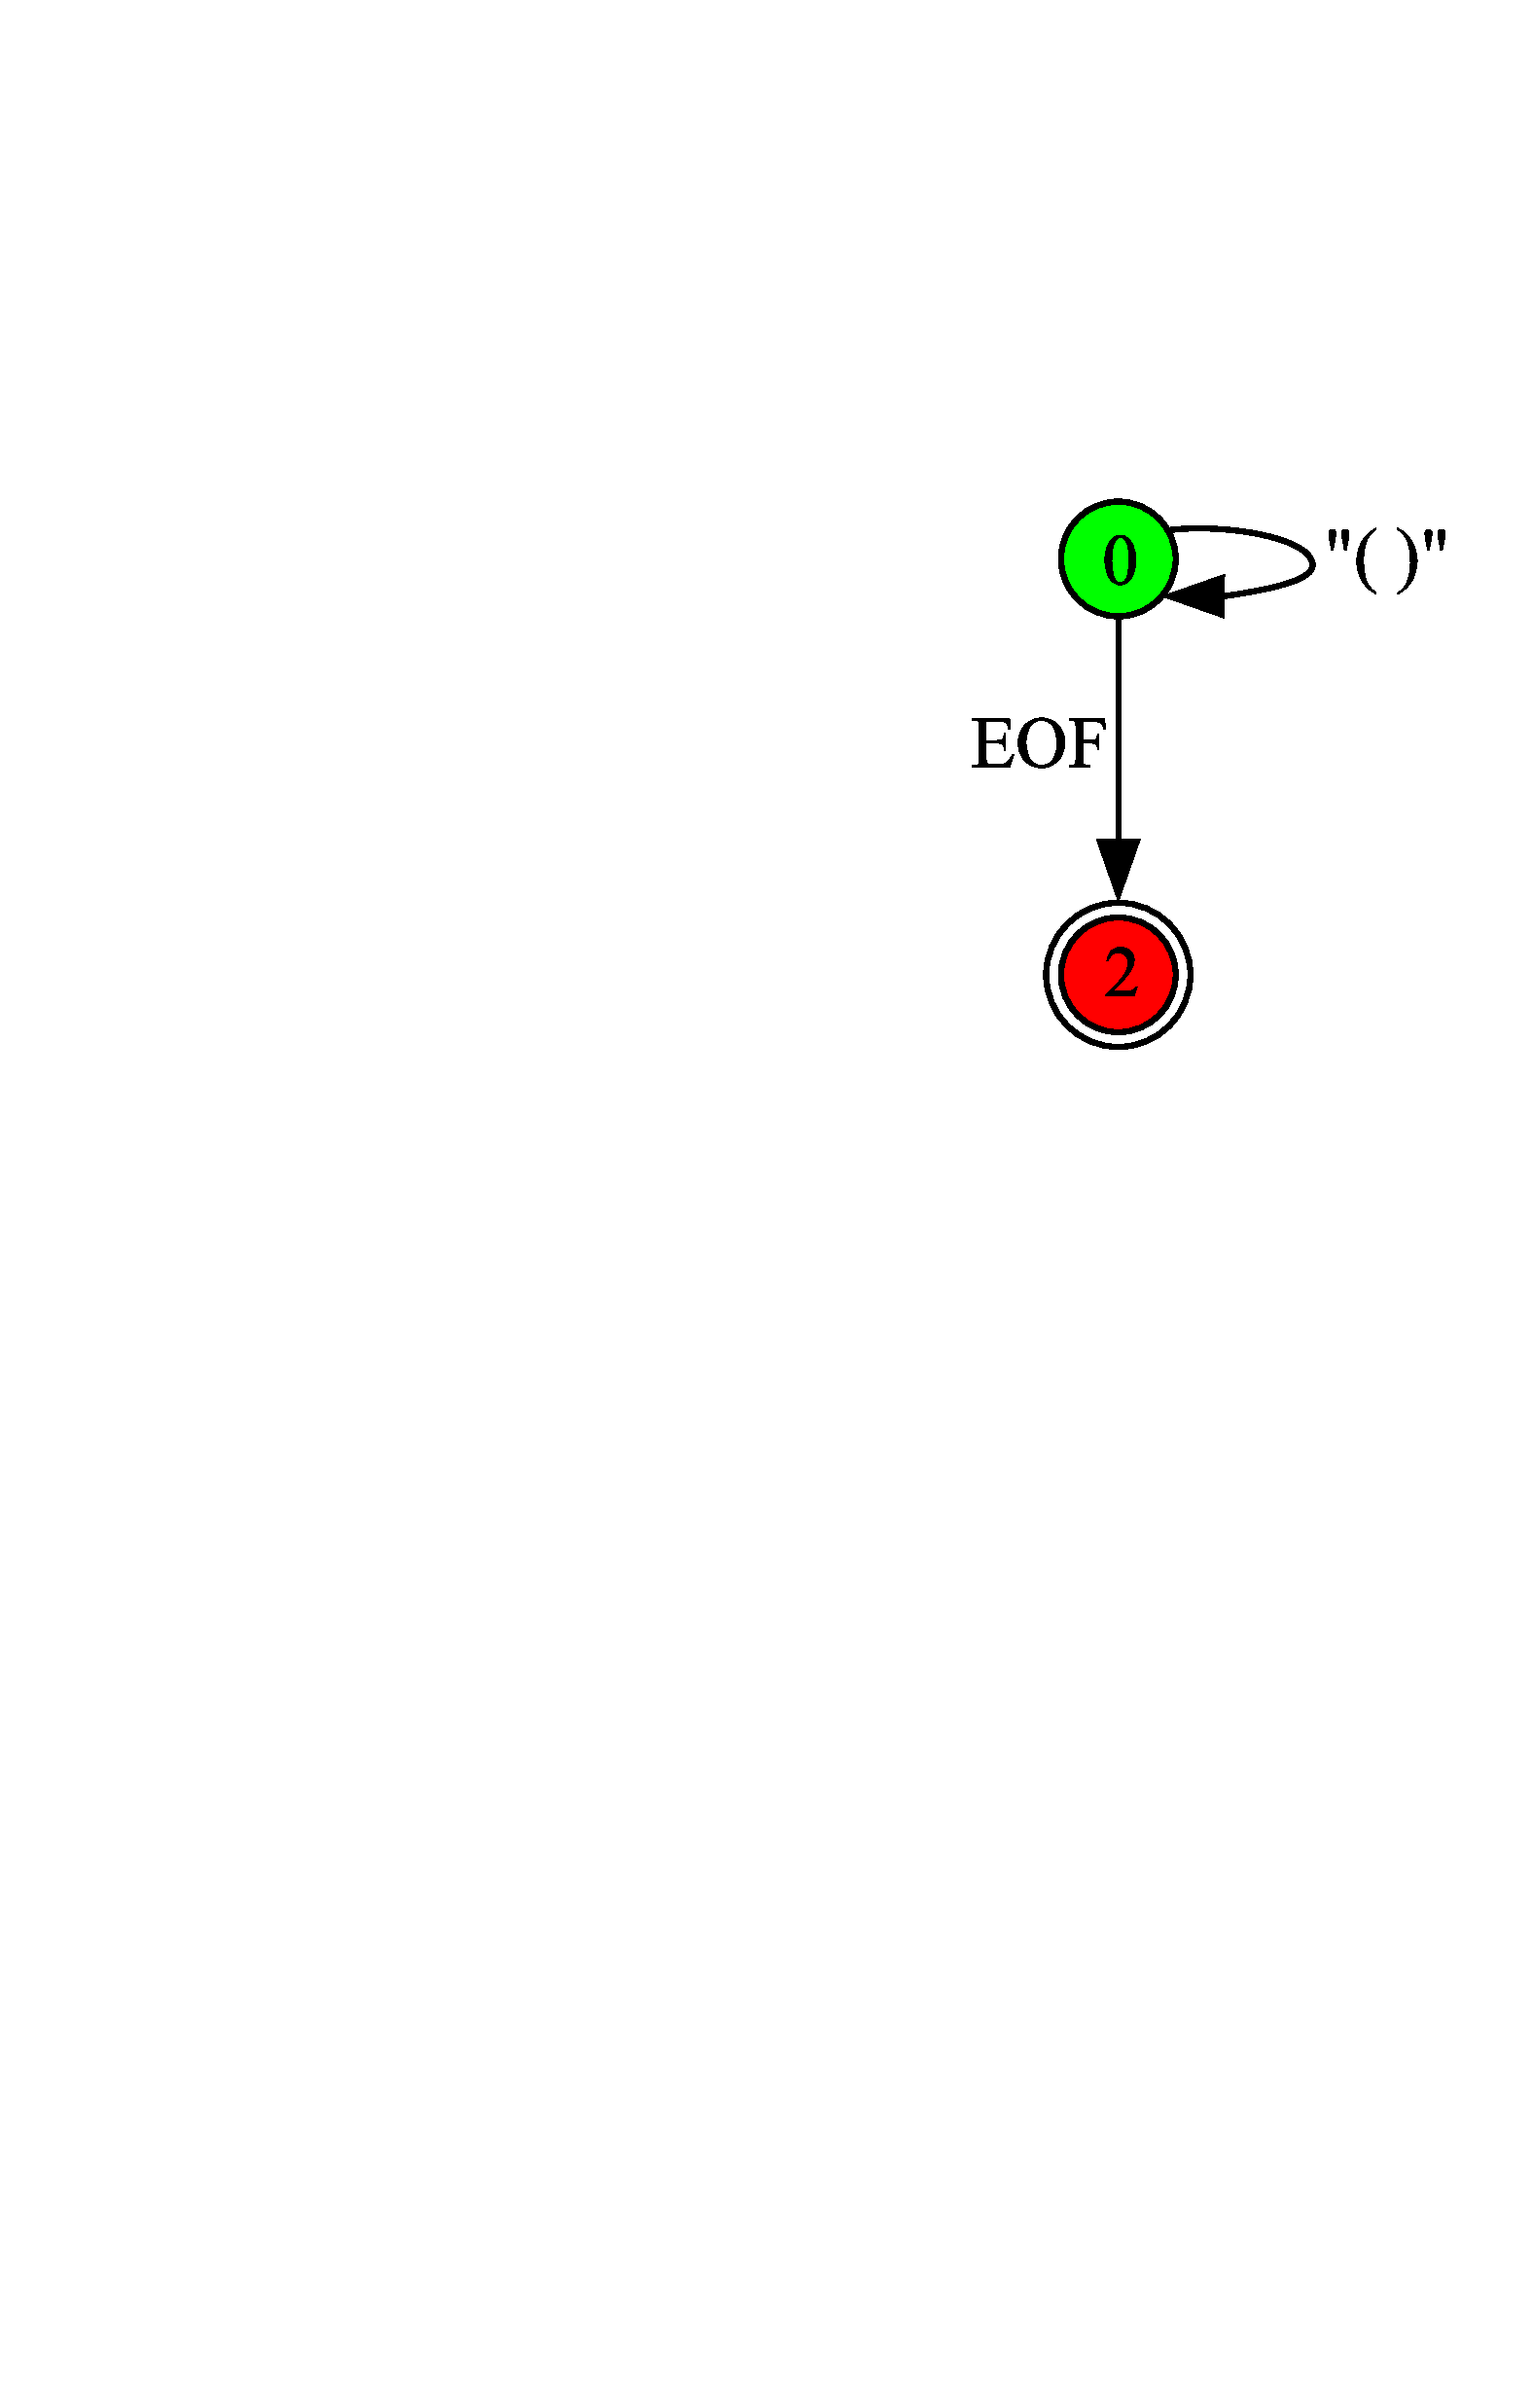
\includegraphics[width=2cm]{pictures/lex1}

lexer\\
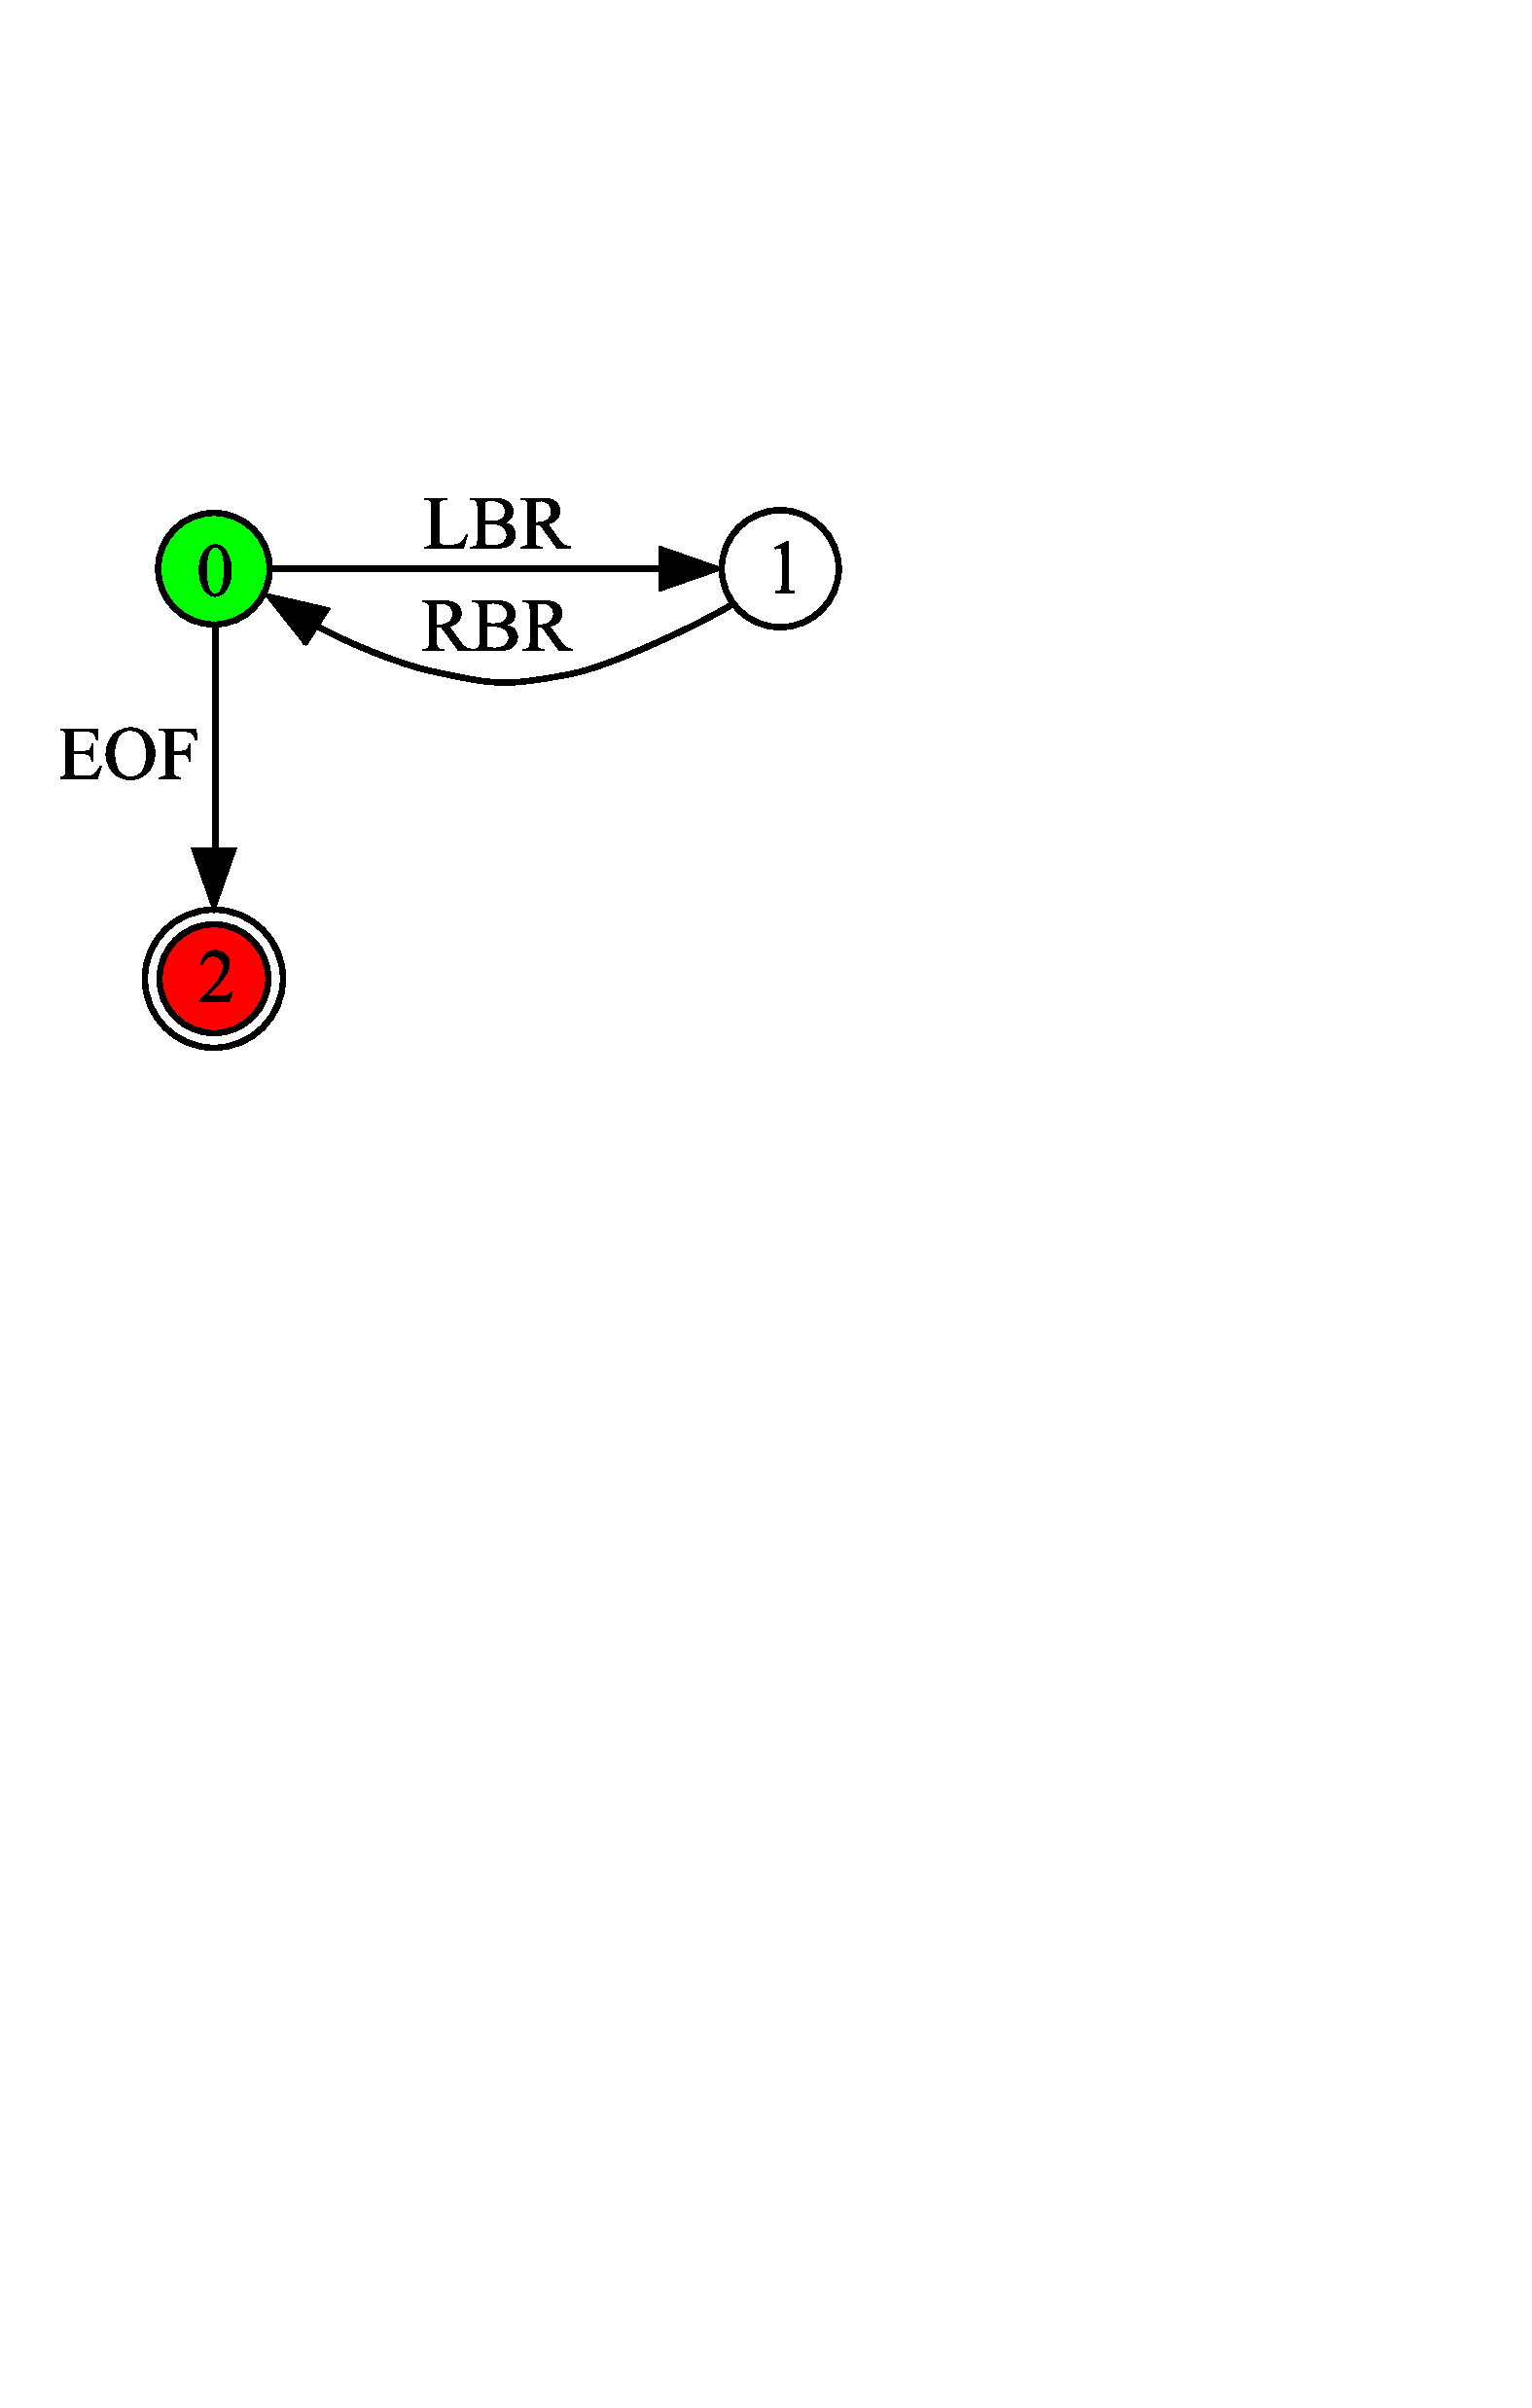
\includegraphics[width=3cm]{pictures/in31}
\end{minipage}
&
\begin{minipage}[t]{8cm}
leser\\
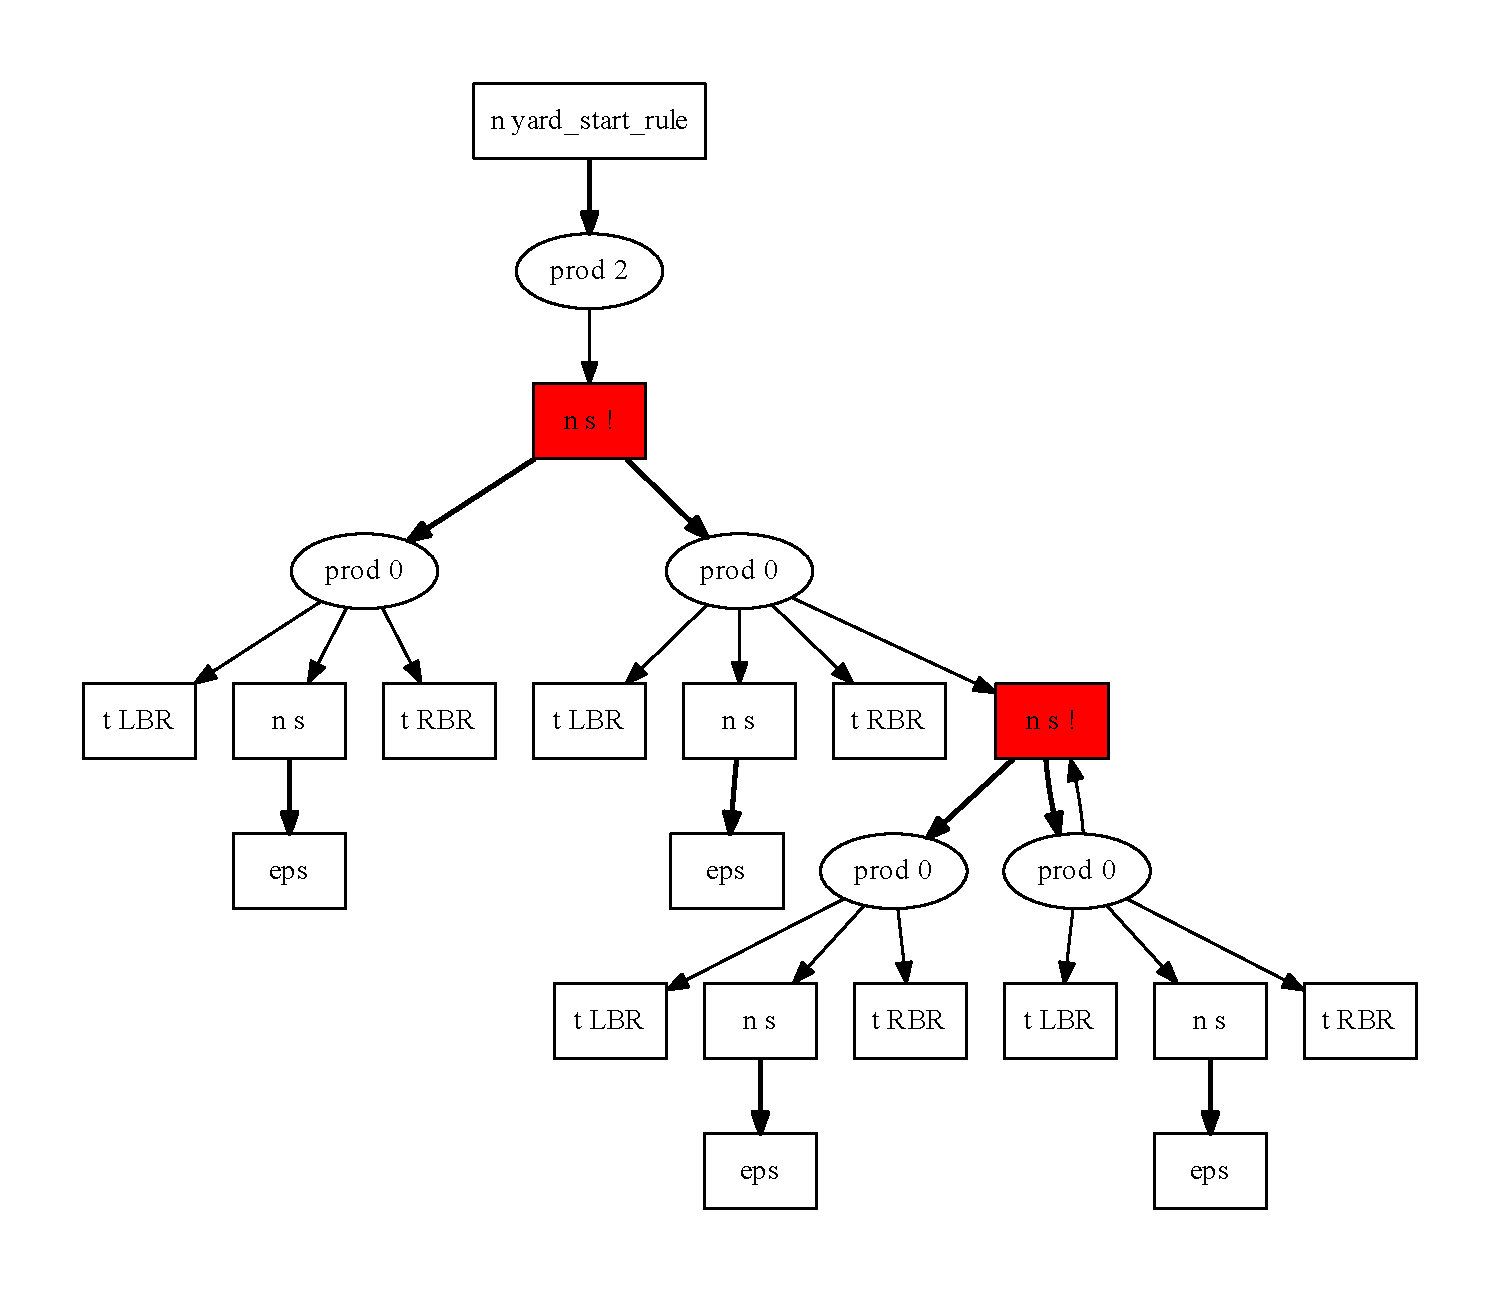
\includegraphics[width=7cm]{pictures/out3}
\end{minipage}

\end{tabular}


\end{frame}



\begin{frame}
  \transwipe[direction=90]
  \frametitle{Existing tools}
  \begin{itemize}
    \item Java String Analyzer, Alvor
    \begin{itemize}
      \item Regular approximation
    \end{itemize}
    \item PHP String Analyzer
    \begin{itemize}
      \item Context-free approximation
    \end{itemize}
    \item Kyung-Goo Doh et al.
    \begin{itemize}
      \item Data flow equations in the domain of LR-stacks
    \end{itemize}
  \end{itemize}
  
  \begin{itemize}
    \item Flaws
    \begin{itemize}
      \item Hard to extend them with new features or support new languages
      \item Do not create structural representation of code
    \end{itemize}
  \end{itemize}
\end{frame}

\begin{frame}
  \transwipe[direction=90]
  \frametitle{Problem statement}
  \textbf{The aim} is to develop the algorithm suitable for syntactic analysis of string-embedded code  
  
  \textbf{Tasks}:
  \begin{itemize}
    \item Develop an algorithm for parsing of regular approximation of embedded 
code which produce a finite parse forest
    \item Parse forest should contain a parse tree for every correct (w.r.t. 
reference grammar) string accepted by the input automaton
    \item Incorrect strings should be omitted: no error detection
  \end{itemize}
\end{frame}
            
\begin{frame}
  \transwipe[direction=90]
  \frametitle{Algorithm}
  \begin{itemize}
    \item \textbf{Input}: reference DCF-grammar $G$ and DFA graph with no 
$\epsilon$-transitions over the alphabeth of terminals of $G$
    \item \textbf{Output}: finite representation of the trees corresponding to 
all correct string accepted by input automaton
  \end{itemize}
\end{frame}

\begin{frame}[fragile]
\transwipe[direction=90]
\frametitle{Algorithm}
\begin{tabular}{p{5cm} p{7cm}}
\begin{minipage}{3in}
  \begin{Verbatim}[commandchars=\\\{\}]

\textcolor{blue}{string} res = \textcolor{orange}{""};
\textcolor{blue}{for}(i = 0; i < l; i++) \{
    res = \textcolor{orange}{"()"} + res;
\}   

  \end{Verbatim}
\end{minipage}
&
Output (SPPF):
\\
Approximation: 
&
\multirow{-2}*{\!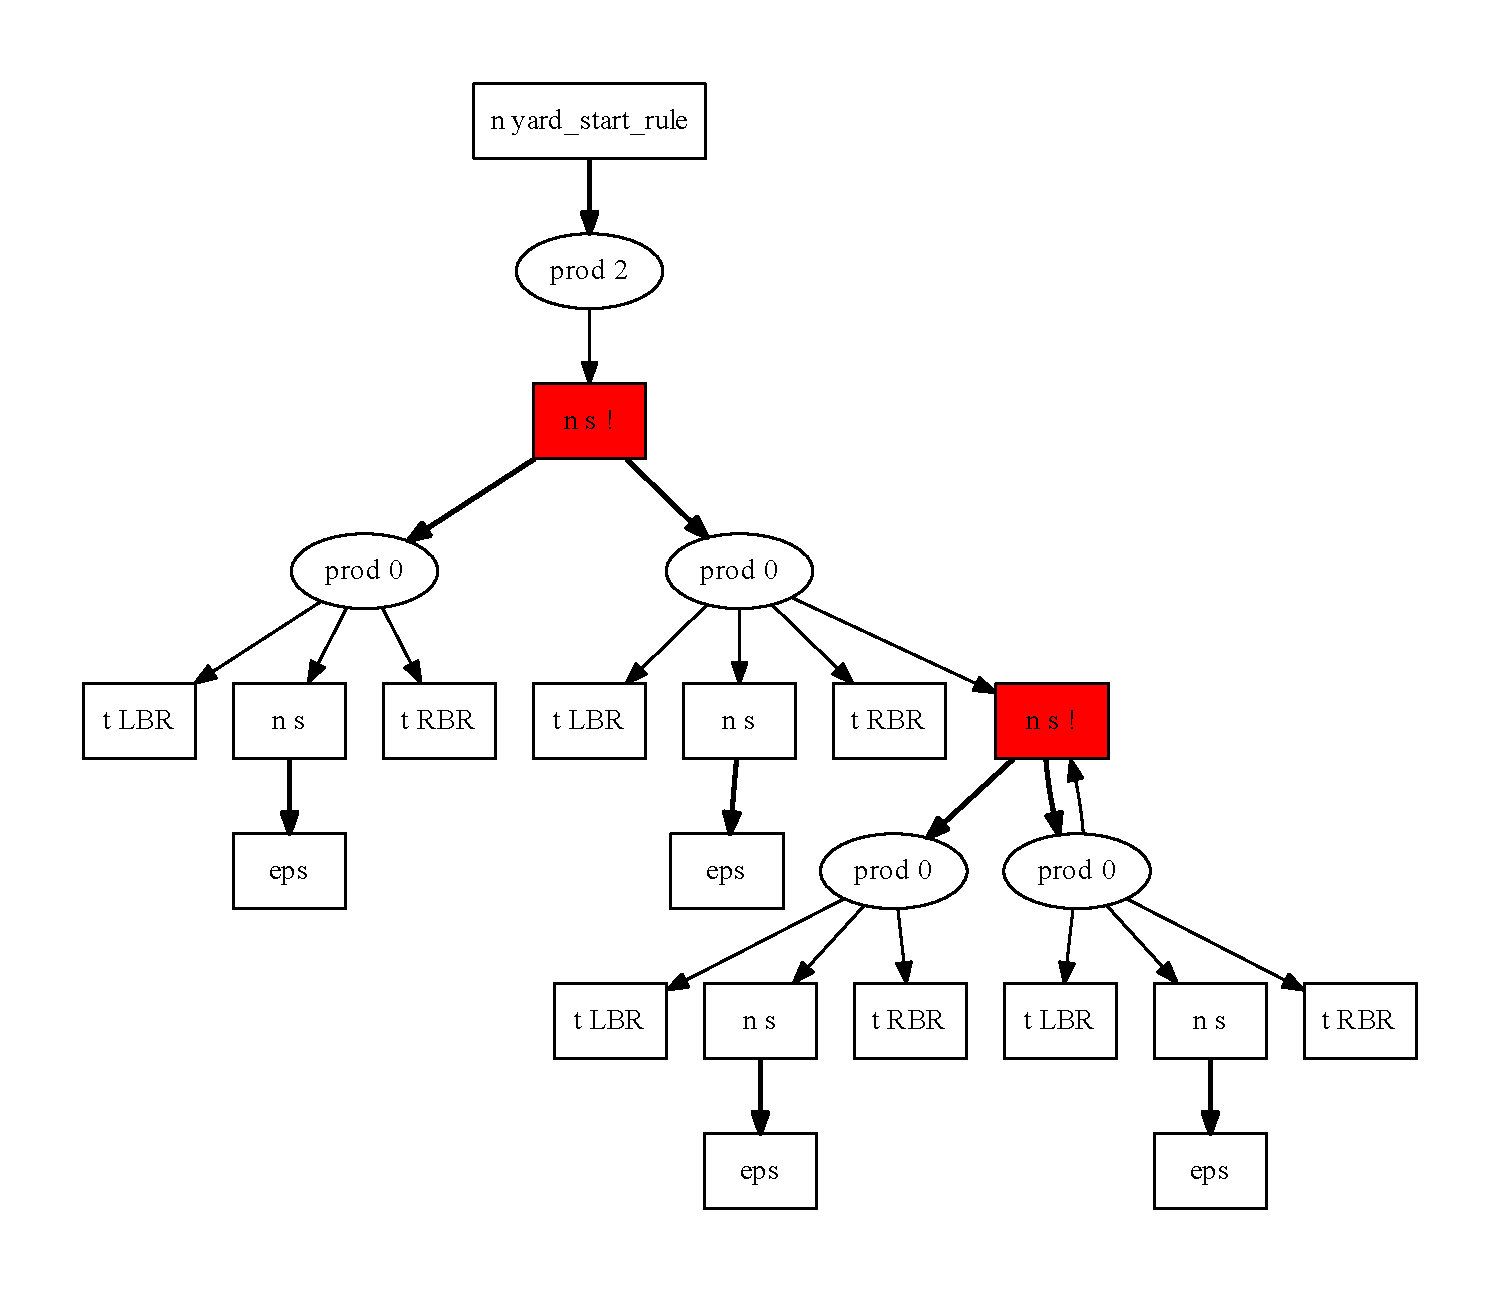
\includegraphics[width=6.8cm]{pictures/out3.pdf}}
\\
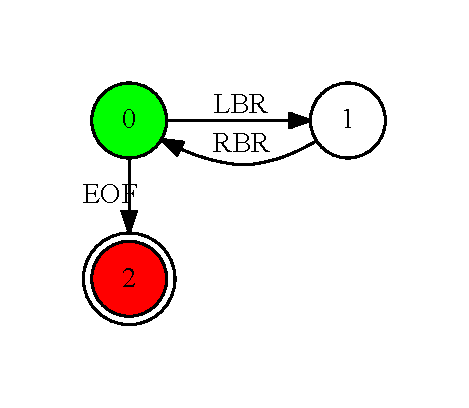
\includegraphics[width=3cm]{pictures/in3.pdf}
&
\\      
Grammar: &
\\
\vspace{-20pt}
$$
\begin{array}{crcl}
&start &::=& s \\
&s & ::= & \mbox{\texttt{LBR }} s \mbox{\texttt{ RBR }} s\\
&s & ::= &\epsilon
\end{array}
$$
& 
\end{tabular}
\end{frame}

\begin{frame}
  \transwipe[direction=90]
  \frametitle{Algorithm}
  \begin{itemize}
    \item Traverse the automaton graph and sequentially construct GSS, similarly as in RNGLR
    \item The set of LR-states is associated with each of input graph vertices
    \item The order in which the vertices of input graph are traversed is 
controled with a queue. The vertex is enqueued whenever new edge with the head 
equal to the vertex is added to the GSS
  \end{itemize}
  \begin{itemize}
    \item The algorithm implements relaxed parsing: errors are not detected, 
erroneous strings are ignored
  \end{itemize}

\end{frame}

\begin{frame}
\transwipe[direction=90]
\frametitle{Algorithm: correctness}
\begin{tabular}{p{5.3cm} p{6.7cm}}
\emph{Correct tree} -- derivation tree of some string accumulated along the 
path in the input graph
&
\\
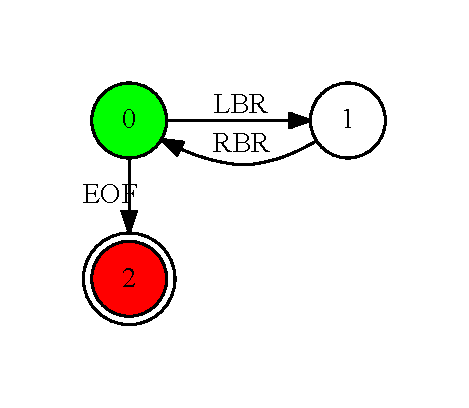
\includegraphics[width=5cm]{pictures/in3.pdf}
&
\includegraphics[width=6cm]{pictures/sppf2.eps}
\end{tabular}
\end{frame}


\begin{frame}
  \transwipe[direction=90]
  \frametitle{Algorithm: correctness}
  \begin{rutheorem}[Termination]
    Algorithm terminates for any input
  \end{rutheorem}
  
  \begin{rutheorem}[Correctness]
    Every tree, generated from SPPF, is correct
  \end{rutheorem}

  \begin{rutheorem}[Correctness]
    For every path $p$ in the inner graph, recognized w.r.t. reference
grammar, a correct tree corresponding to $p$ can be generated from SPPF
  \end{rutheorem}
\end{frame}

\begin{frame}
  \transwipe[direction=90]
  \frametitle{Implementation}
  \begin{itemize}
    \item The algorithm is implemented as a part of YaccConstructor project 
using F\# programming language
    \item The generator of RNGLR parse tables and data structures for GSS and 
SPPF are reused
 \end{itemize}
\end{frame}

\begin{frame}[t]
  \transwipe[direction=90]
  \frametitle{Evaluation}
  \begin{itemize}
    \item The data is taken from the project of migration from MS-SQL to Oracle Server 
    \item 2,7 lines of code, 2430 queries, 2188 successfully processed
    \item The number of queries which previously could not be processed because 
of timeout is decreased from 45 to 1
  \end{itemize}
  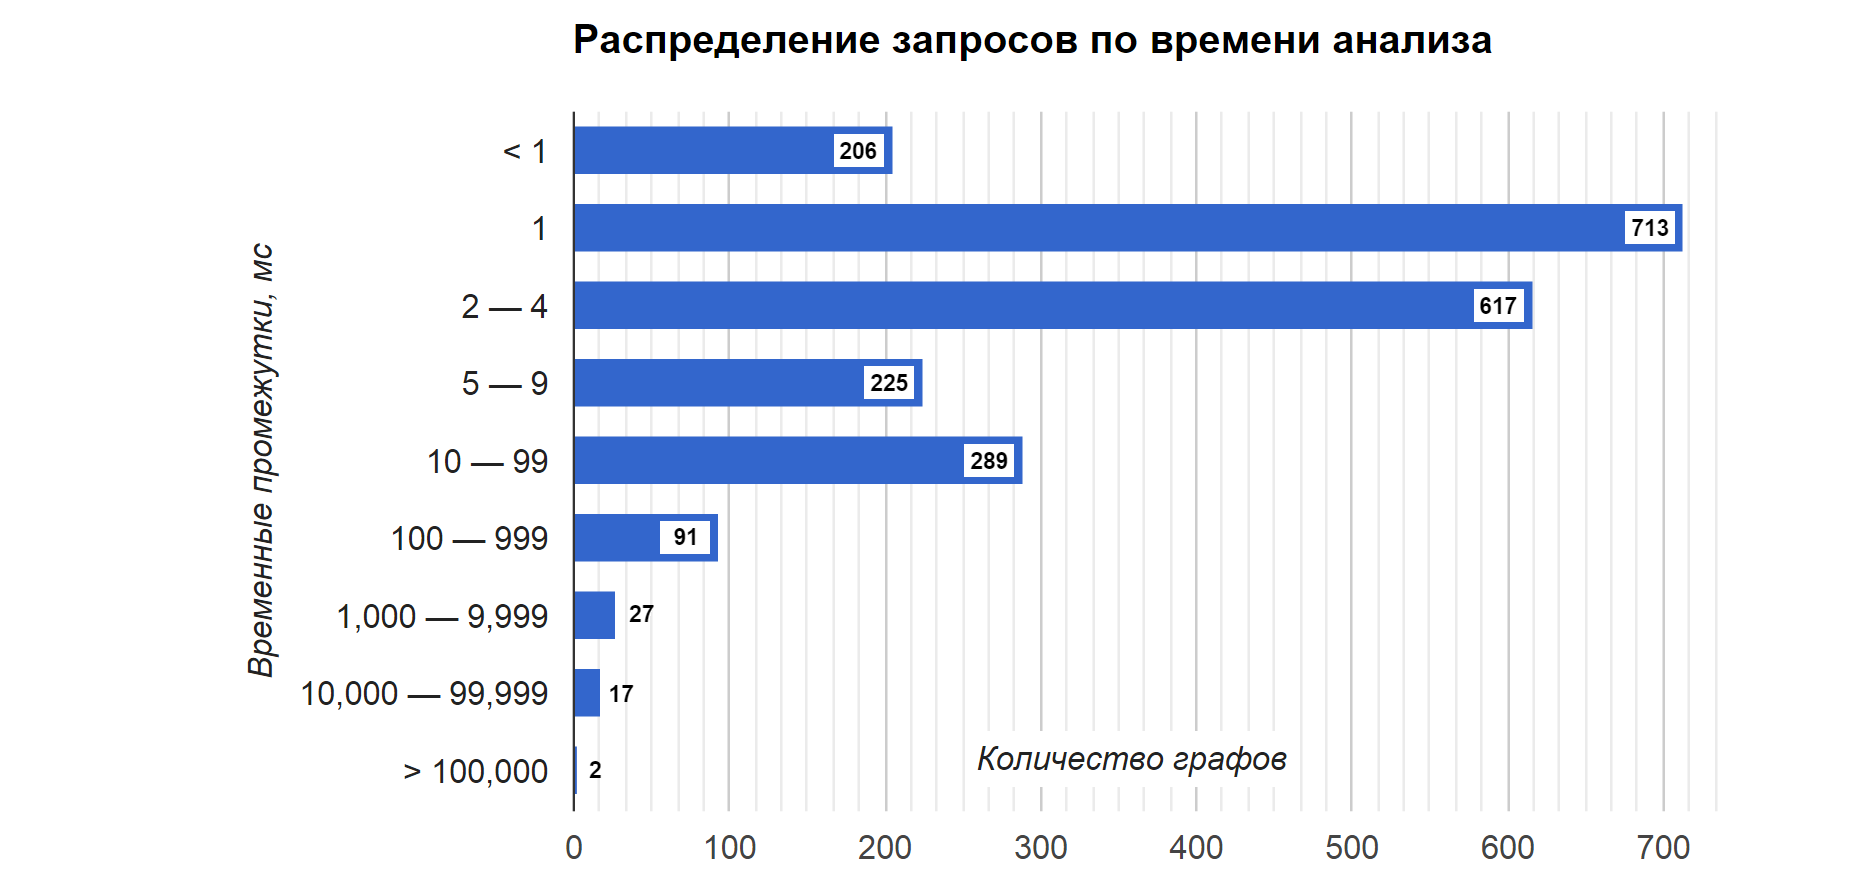
\includegraphics[width=10cm]{pictures/dist.png}
\end{frame}


\begin{frame}
  \transwipe[direction=90]
  \frametitle{Conclusion}
  \begin{itemize}
    \item The algorithm for parsing of regular approximation of dynamically 
generated string which constructs the finite representation of parse forest is 
developped
    \item Its termination and correctness are proved
    \item The algorithm is implemented as a part of YaccConstructor project
    \item The evaluation demonstrated it could be used for complex tasks
  \end{itemize}
\end{frame}

\end{document}
